\begin{example}
  \vspace{-1em}
  \begin{align*}
      A_1 & =
      \begin{bmatrix}
          0 & 2\\
          0 & 0
      \end{bmatrix}&
      A_2 & =
      \begin{bmatrix}
          0 & 0\\
          2 & 0
      \end{bmatrix}
  \end{align*}
  \vspace{-2em}
  \begin{center}
    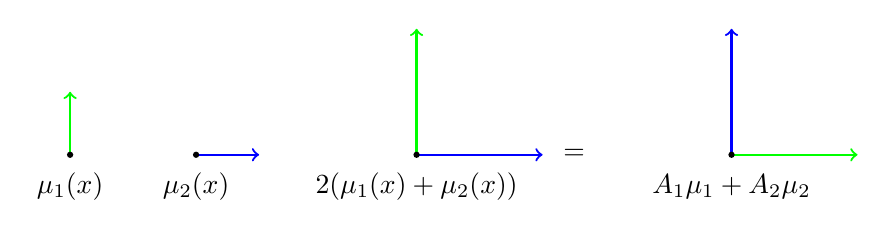
\begin{tikzpicture}[scale=0.8]
        \begin{scope}[shift={(-8,0)}]
            \draw[thick,->,green] (0,0) to (0,1);
            \fill (0,0) circle(.05);
            \node at (0,-.5) {$\mu_1(x)$};
        \end{scope}

        \begin{scope}[shift={(-6,0)}]
            \draw[thick,->,blue] (0,0) to (1,0);
            \fill (0,0) circle(.05);
            \node at (0,-.5) {$\mu_2(x)$};
        \end{scope}

        \begin{scope}[shift={(-2.5,0)}]
            \draw[thick,->,green] (0,0) to (0,2);
            \draw[thick,->,blue] (0,0) to (2,0);
            \fill (0,0) circle(.05);
            \node at (0,-.5) {$2(\mu_1(x) + \mu_2(x))$};
        \end{scope}

        \begin{scope}[shift={(0,0)}]
            \node at (0,0) {$=$};
        \end{scope}

        \begin{scope}[shift={(2.5,0)}]
            \draw[thick,->,green] (0,0) to (2,0);
            \draw[thick,->,blue] (0,0) to (0,2);
            \fill (0,0) circle(.05);
            \node at (0,-.5) {$\pushf{A_1}{\mu_1} + \pushf{A_2}{\mu_2}$};
        \end{scope}
    \end{tikzpicture}
  \end{center}
\end{example}
